% Name: Aggregate demand and supply
% Description: Aggregate demand shifts right from AD₁ to AD₂: in the short run the economy moves up the SRAS curve to higher output and prices, past the potential output marked by LRAS.
% Tags: aggregate demand, aggregate supply, AD-AS model, macroeconomics

\usetikzlibrary{arrows.meta}

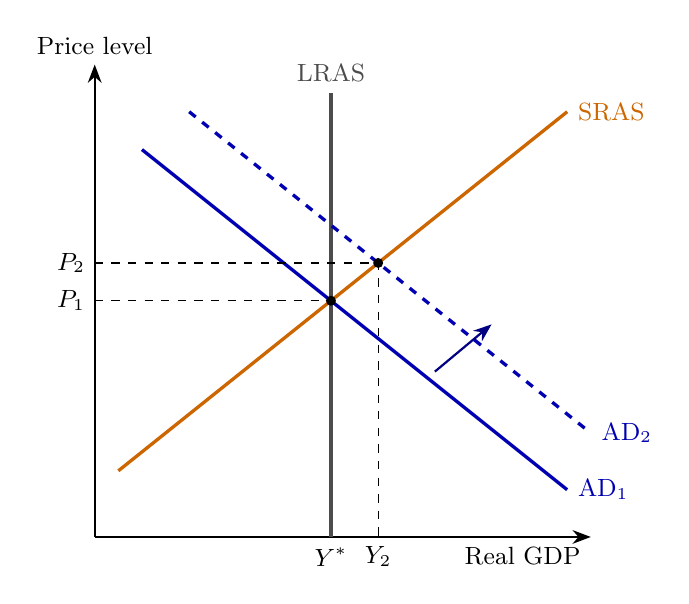
\begin{tikzpicture}[>={Stealth}, scale=0.6, every node/.style={font=\small}]
  % SRAS: P = 1 + 0.8Y, AD₁: P = 9 - 0.8Y, AD₂: P = 10.6 - 0.8Y; AD₁ meets SRAS at (5, 5) on LRAS, AD₂ at (6, 5.8)
  \draw[->, thick] (0,0) -- (10.5,0) node[below left] {Real GDP};
  \draw[->, thick] (0,0) -- (0,10) node[above] {Price level};
  \draw[very thick, gray!60!black] (5,0) node[below, black] {$Y^*$} -- (5,9.4) node[above] {LRAS};
  \draw[very thick, orange!80!black] (0.5,1.4) -- (10,9) node[right] {SRAS};
  \draw[very thick, blue!70!black] (1,8.2) -- (10,1) node[right] {AD$_1$};
  \draw[very thick, blue!70!black, dashed] (2,9) -- (10.5,2.2) node[right] {AD$_2$};
  \draw[->, thick, blue!50!black] (7.2,3.5) -- (8.4,4.5);
  \draw[dashed] (0,5) node[left] {$P_1$} -- (5,5);
  \draw[dashed] (0,5.8) node[left] {$P_2$} -| (6,0) node[below] {$Y_2$};
  \fill (5,5) circle (3pt) (6,5.8) circle (3pt);
\end{tikzpicture}
